\section{Implementation}

We have implemented the Kernel Principal Component Analysis method in Matlab. We have used the results from Kernel PCA in a classification problem using two different linear classifiers.

The algorithm which we have implemented is,

\begin{enumerate}
    \item Compute the matrix \textbf{K} (\ref{eq:k_matrix}) using a kernel function
    \item Solve equation (\ref{eq:solution}) by diagonalizing \textbf{K}
    \item Solve equation (\ref{eq:alpha_coeff}) to compute the $\boldsymbol{\alpha}^k$ coefficients normalizing the corresponding eigenvectors
    \item Project a test point onto the principal components
\end{enumerate}

We have implemented the algorithm in two functions. One function that takes in a training data set and computes the matrix \textbf{K} using a polynomial kernel, finds the expansion coefficients $\boldsymbol{\alpha}^k$ and projects the training data onto the eigenvectors. It then returns $\boldsymbol{\alpha}^k$ as well as the projected training data. The second function  takes in a test data set and projects it onto the eigenvectors extracted from the training data	.

We then perform classification using the two sets of projected data, training and test data. We train the two classifiers on the projected training data and then test it in on the projected testing data.
The first classifier used are the built in Matlab function \texttt{classify} which fits a Multivariate Gaussian to each of the clusters and that way create a linear classifier. The other classifier that we have used is a Support Vector Machine classifier implemented in LIBSVM \cite{CC01a} where we have used the linear implementation.

\subsection{Experiment}
We have evaluated the performance of our implementation of the Kernel PCA with a classification problem. We are considering the USPS (US Postal Service) handwritten digit dataset. It consists of 9300 observations each of 256 dimensions where each dimension is a pixel in a gray scale image of a handwritten digit of $16\times 16$ pixels. 
Each observation is associated with a label describing the handwritten digit. The test set is made up by 2000 observations and here we use 3000 observation for our training set. 

We have then extracted the principal components from the training and test data sets as described above and trained a separating hyperplane classifier on this projection of the training data. After that we have tested the classifier using the projected testing data.

We have used a polynomial kernel of degree, $d = 1,\dots,6$, and extracted the first $2^n$, $n = 6,7,\dots,11$, principal components.

In these experiments we have used two different kinds of linear classifier. The first we have used is the Matlab function \texttt{classify}. It fits a Multivariate Gaussian to each of the 10 clusters and creates the classification boundaries. The results using this classifier are shown in Figure \ref{fig:GMM}. Here, we can see that for polynomial degree $d=1$ the best classification performance is for 128 principal components with an error of 8.2\%. This corresponds well with the results obtained in \citep{scholkopf1997kernel} where they get 8.6\% error for this combination. Further, we see that in all other cases of 128 non-linear components, that is $d=2,\dots,6$, give a better performance with an error around 5 to 6\%. Again this corresponds well with the results in the original article. We also see that extracting more principal components leads to even better performances for $d>2$ and with 2048 principal components we get an error of about 2.5\%. So generally the pattern that our results show corresponds well with the results in the original article.

\begin{figure}
    \centering
    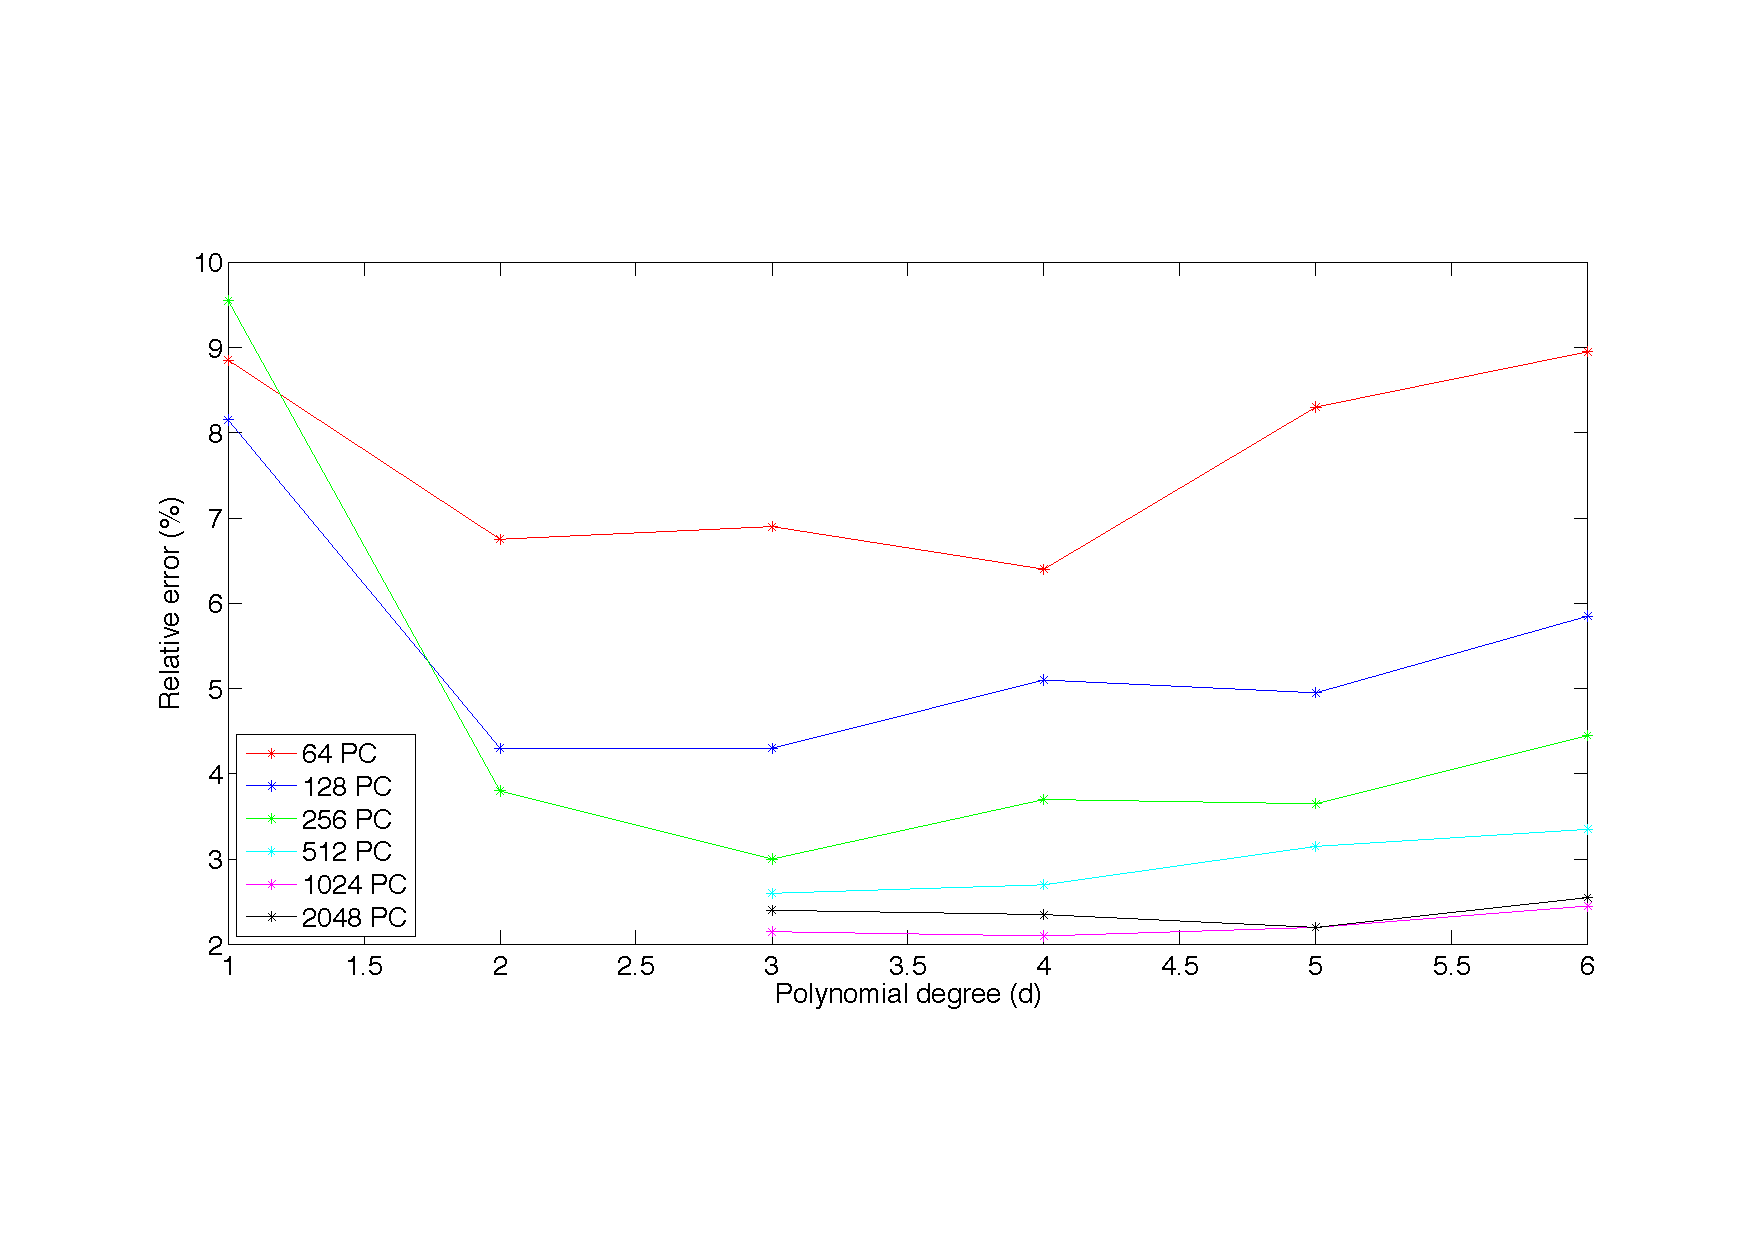
\includegraphics[width=\textwidth]{img/errorplotGMMclass.pdf}
    \caption{Classification errors using \texttt{classify} for different degrees of polynomial kernel and different numbers of principal components. The classification for a number of principal components higher than the dimension of the observations was only possible for polynomial degree $d>2$.}
    \label{fig:GMM}
\end{figure}

However, in the article \citep{scholkopf1997kernel} they used a linear Support Vector Machine (SVM) classifier and not just any linear classifier. The results using linear SVM can be seen in Figure \ref{fig:SVM}. Here we see that the best classification performance for linear PCA, $d=1$, was reached for 512 principal components and that was 6.6\%. The worst performance for $d=1$ was with 64 principal components with an error of 7.3\%. We notice that even the worst performance is better than the best performance we found for the previous classifier. If we then consider higher polynomial degrees $d>1$, we notice that the best performance for all numbers of principal components is achieved at polynomial degree 3 or 4 depending on the number of principal components extracted and for degrees higher than that the error increases again. Overall the level of error corresponds well with the original article's results but we do not get the same pattern in the results as we got for the previous classifier.
Also, since we do not know which type of multiclass SVM was used, one-vs-all or one-vs-one, whether a slack was used or not and how large and how compliant was the slack, we could not reproduce the exact results described in the paper.

\begin{figure}
    \centering
    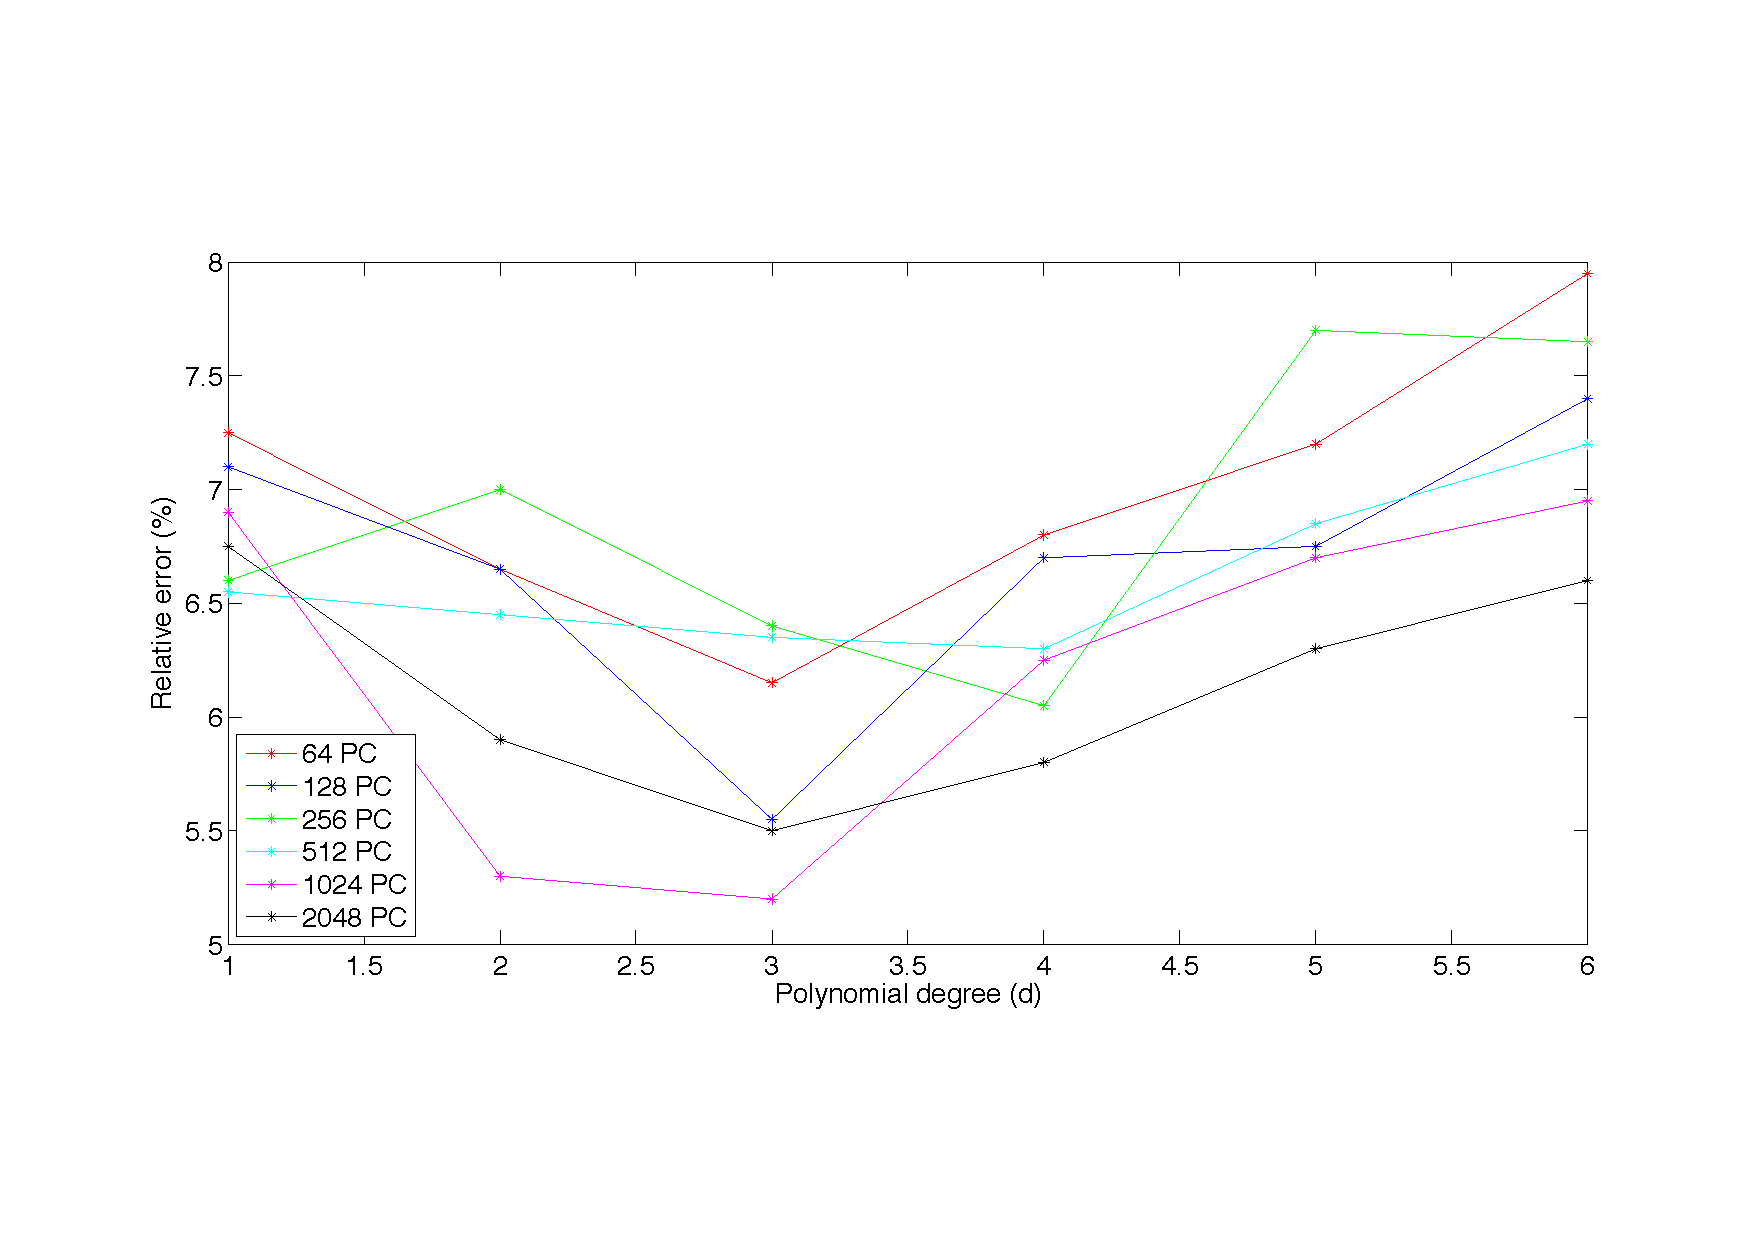
\includegraphics[width=\textwidth]{img/errorplotSVMclass.pdf}
    \caption{Classification errors using linear SVM classifier for different degrees of polynomial kernel and different numbers of principal components.}
    \label{fig:SVM}
\end{figure}


Generally, we were able to recreate their experiment even though all our error rates do not correspond exactly to the ones obtained in the original article. This can be due to differences in the linear classifiers because of different parameters or simply improvements in the implementations of these classifiers since the article was published in 1997.